\documentclass[10pt,tikz,border=6pt]{standalone}
\usetikzlibrary{arrows.meta,positioning}
\begin{document}
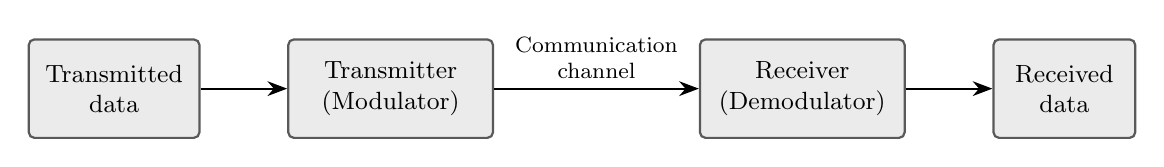
\begin{tikzpicture}[
  font=\small,
  block/.style={draw=black!65,fill=black!8,rounded corners=2pt,
    line width=0.8pt,minimum height=1.25cm,align=center,inner sep=6pt},
  connection/.style={-{Stealth[length=2.5mm]},line width=0.8pt}
]
\node[block,minimum width=1.8cm] (input) {Transmitted\\data};
\node[block,minimum width=2.6cm,right=1.1cm of input] (tx) {Transmitter\\(Modulator)};
\node[block,minimum width=2.6cm,right=2.6cm of tx] (rx) {Receiver\\(Demodulator)};
\node[block,minimum width=1.8cm,right=1.1cm of rx] (output) {Received\\data};
\draw[connection] (input) -- (tx);
\draw[connection] (tx) -- node[above,align=center,font=\footnotesize] {Communication\\channel} (rx);
\draw[connection] (rx) -- (output);
\end{tikzpicture}
\end{document}
